\documentclass{beamer}

\usepackage{graphicx}
\usepackage{amsmath}
\usepackage{booktabs}

\title{Parallel Ant Colony Optimization on Multi-Core CPUs}
\subtitle{Accelerating the TSP Solution}
\author{Douglas Sousa Jorge, Isaac Brasil Oliveira}
\institute{INF - UFG}
\date{}

\begin{document}
	
	\frame{\titlepage}
	
	\begin{frame}
		\frametitle{Problema}
		\begin{itemize}
			\item A Otimização por Colônia de Formigas (ACO) é uma meta-heurística popular para resolver problemas de otimização combinatória, como o Problema do Caixeiro Viajante (TSP).
			\item Implementações sequenciais de ACO são frequentemente limitadas pelo tempo de execução, especialmente em problemas de grande escala.
			\item Paralelizar o ACO pode melhorar significativamente a eficiência, mas apresenta desafios em termos de acesso e controle de dados.
		\end{itemize}
	\end{frame}
	
	\begin{frame}
		\frametitle{Solução Proposta}
		\begin{itemize}
			\item Proposta de um novo modelo de ACO paralelo para arquitetura de CPU multi-core.
			\item Introdução de uma abordagem de seleção proporcional à aptidão chamada Roda da Roleta Vetorial (VRW).
			\item Utilização de instruções vetoriais para acelerar a construção do tour de cada formiga.
		\end{itemize}
	\end{frame}
	
	\begin{frame}
		\frametitle{Metodologia}
		\begin{itemize}
			\item \textbf{Inicialização:}
			\begin{itemize}
				\item Matrizes de distâncias, feromônios e heurísticas são inicializadas aleatoriamente.
			\end{itemize}
			\item \textbf{Construção de Solução:}
			\begin{itemize}
				\item Cada formiga constrói um tour baseado nos feromônios e nas heurísticas utilizando a VRW.
			\end{itemize}
			\item \textbf{Atualização de Feromônios:}
			\begin{itemize}
				\item Feromônios são atualizados com base nos tours construídos pelas formigas.
			\end{itemize}
			\item \textbf{Medição de Tempo:}
			\begin{itemize}
				\item Tempo de execução é medido para diferentes números de iterações (\(n\)).
			\end{itemize}
		\end{itemize}
	\end{frame}
	
	\begin{frame}
		\frametitle{Metodologia}
		\begin{itemize}
			\item \textbf{Hardware utilizado:}
			\begin{itemize}
				\item CPU: AMD Ryzen 5 5600 (6/12)
				\item GPU: AMD Radeon RX 6750 XT
				\item RAM: 16gb ddr4 3600mhz
			\end{itemize}
		\end{itemize}
	\end{frame}
	
	\begin{frame}
		\frametitle{Solução}
		\begin{figure}
			\centering
			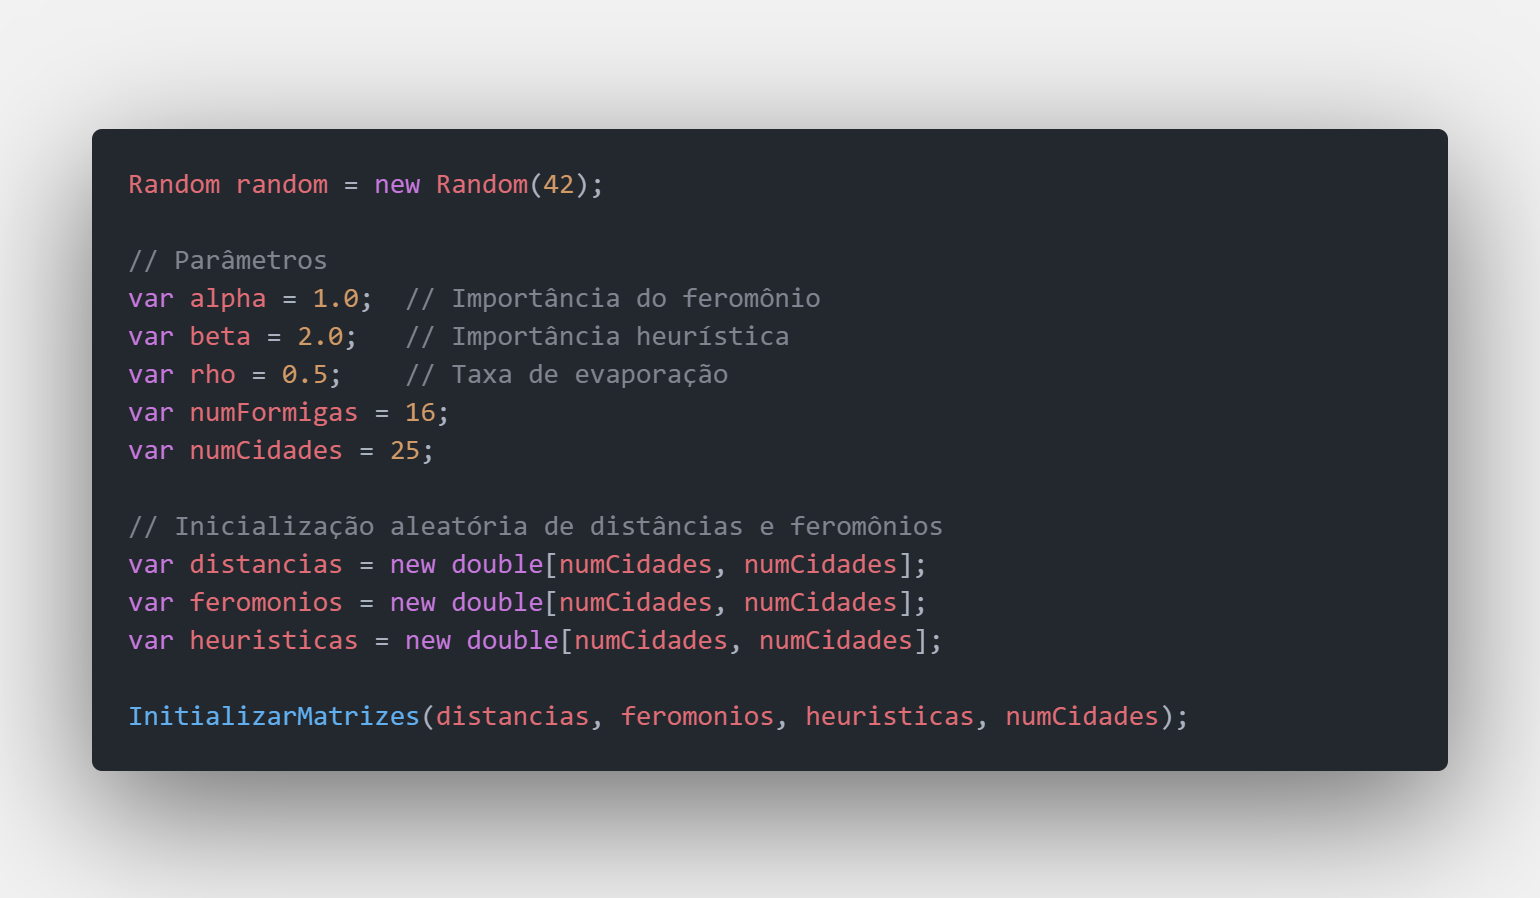
\includegraphics[width=1\linewidth]{code definition.png} % Substitua "execution_times.png" pelo caminho da sua imagem
			\caption{Definições do programa}
		\end{figure}
	\end{frame}
	
	\begin{frame}
		\frametitle{Solução}
		\begin{figure}
			\centering
			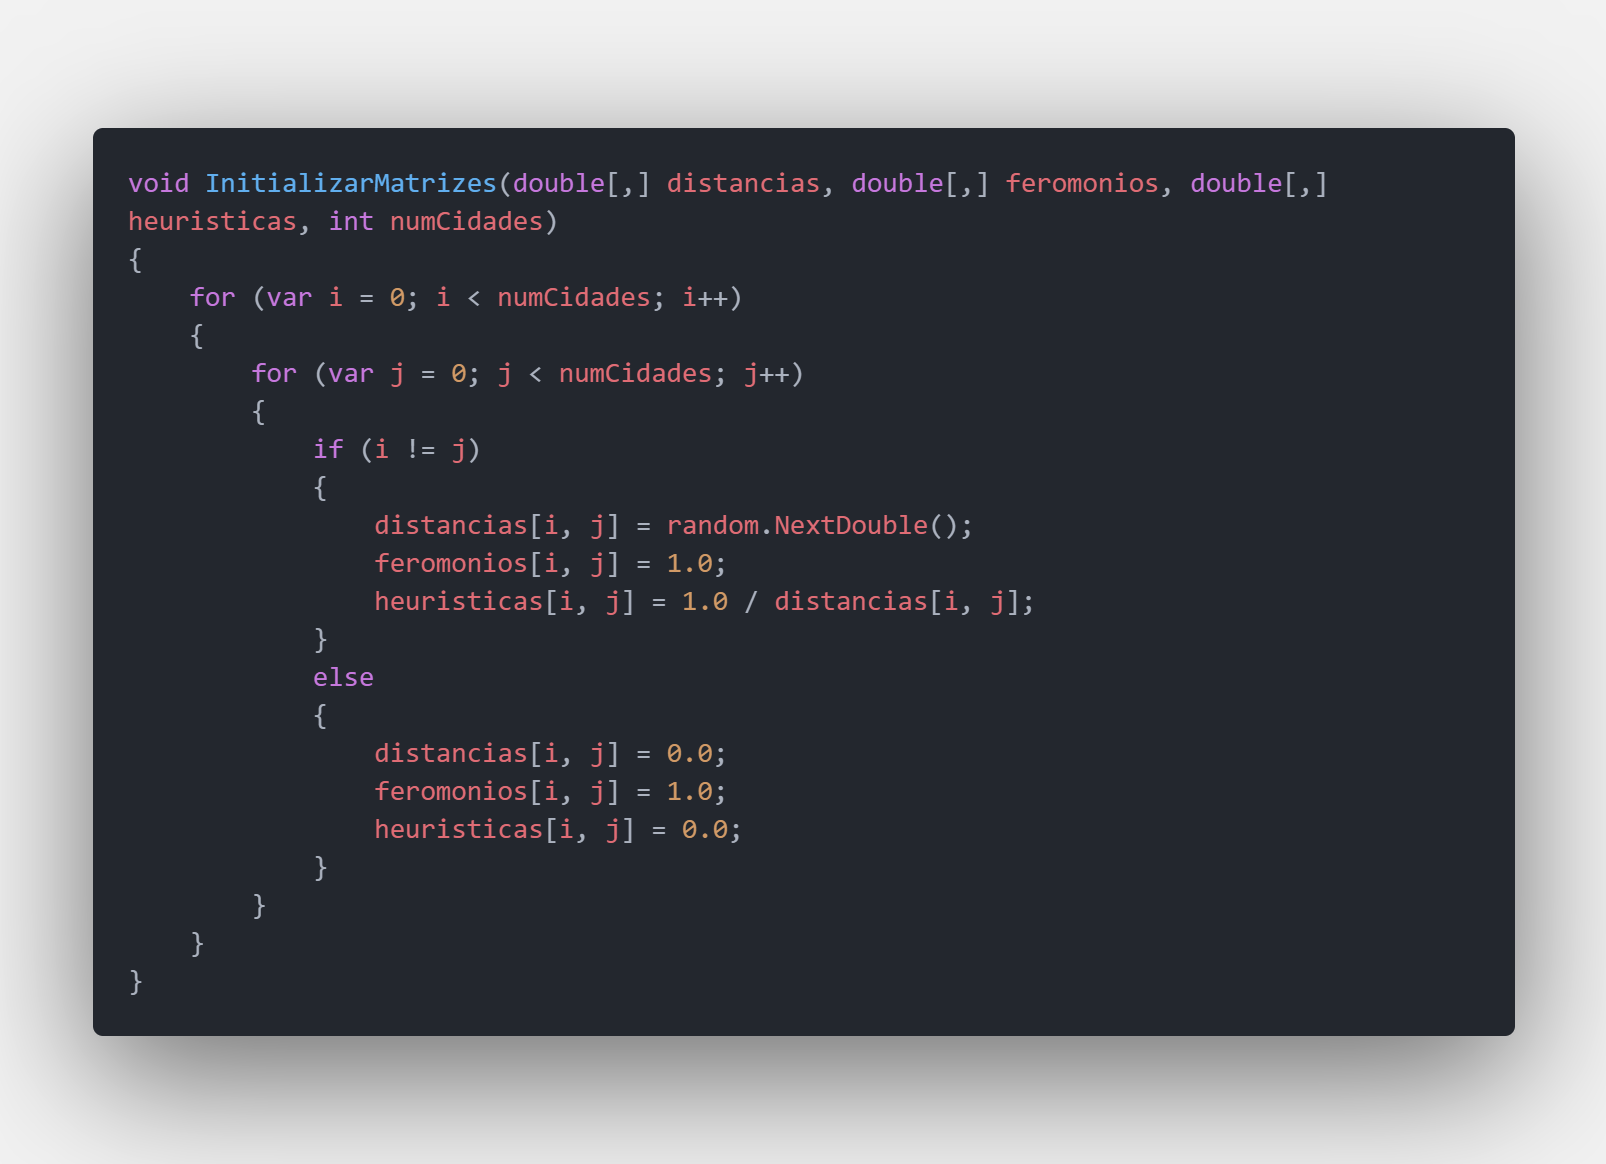
\includegraphics[width=.8\linewidth]{code initialization.png} % Substitua "execution_times.png" pelo caminho da sua imagem
			\caption{Inicialização das matrizes}
		\end{figure}
	\end{frame}
	
	\begin{frame}
		\frametitle{Solução}
		\begin{figure}
			\centering
			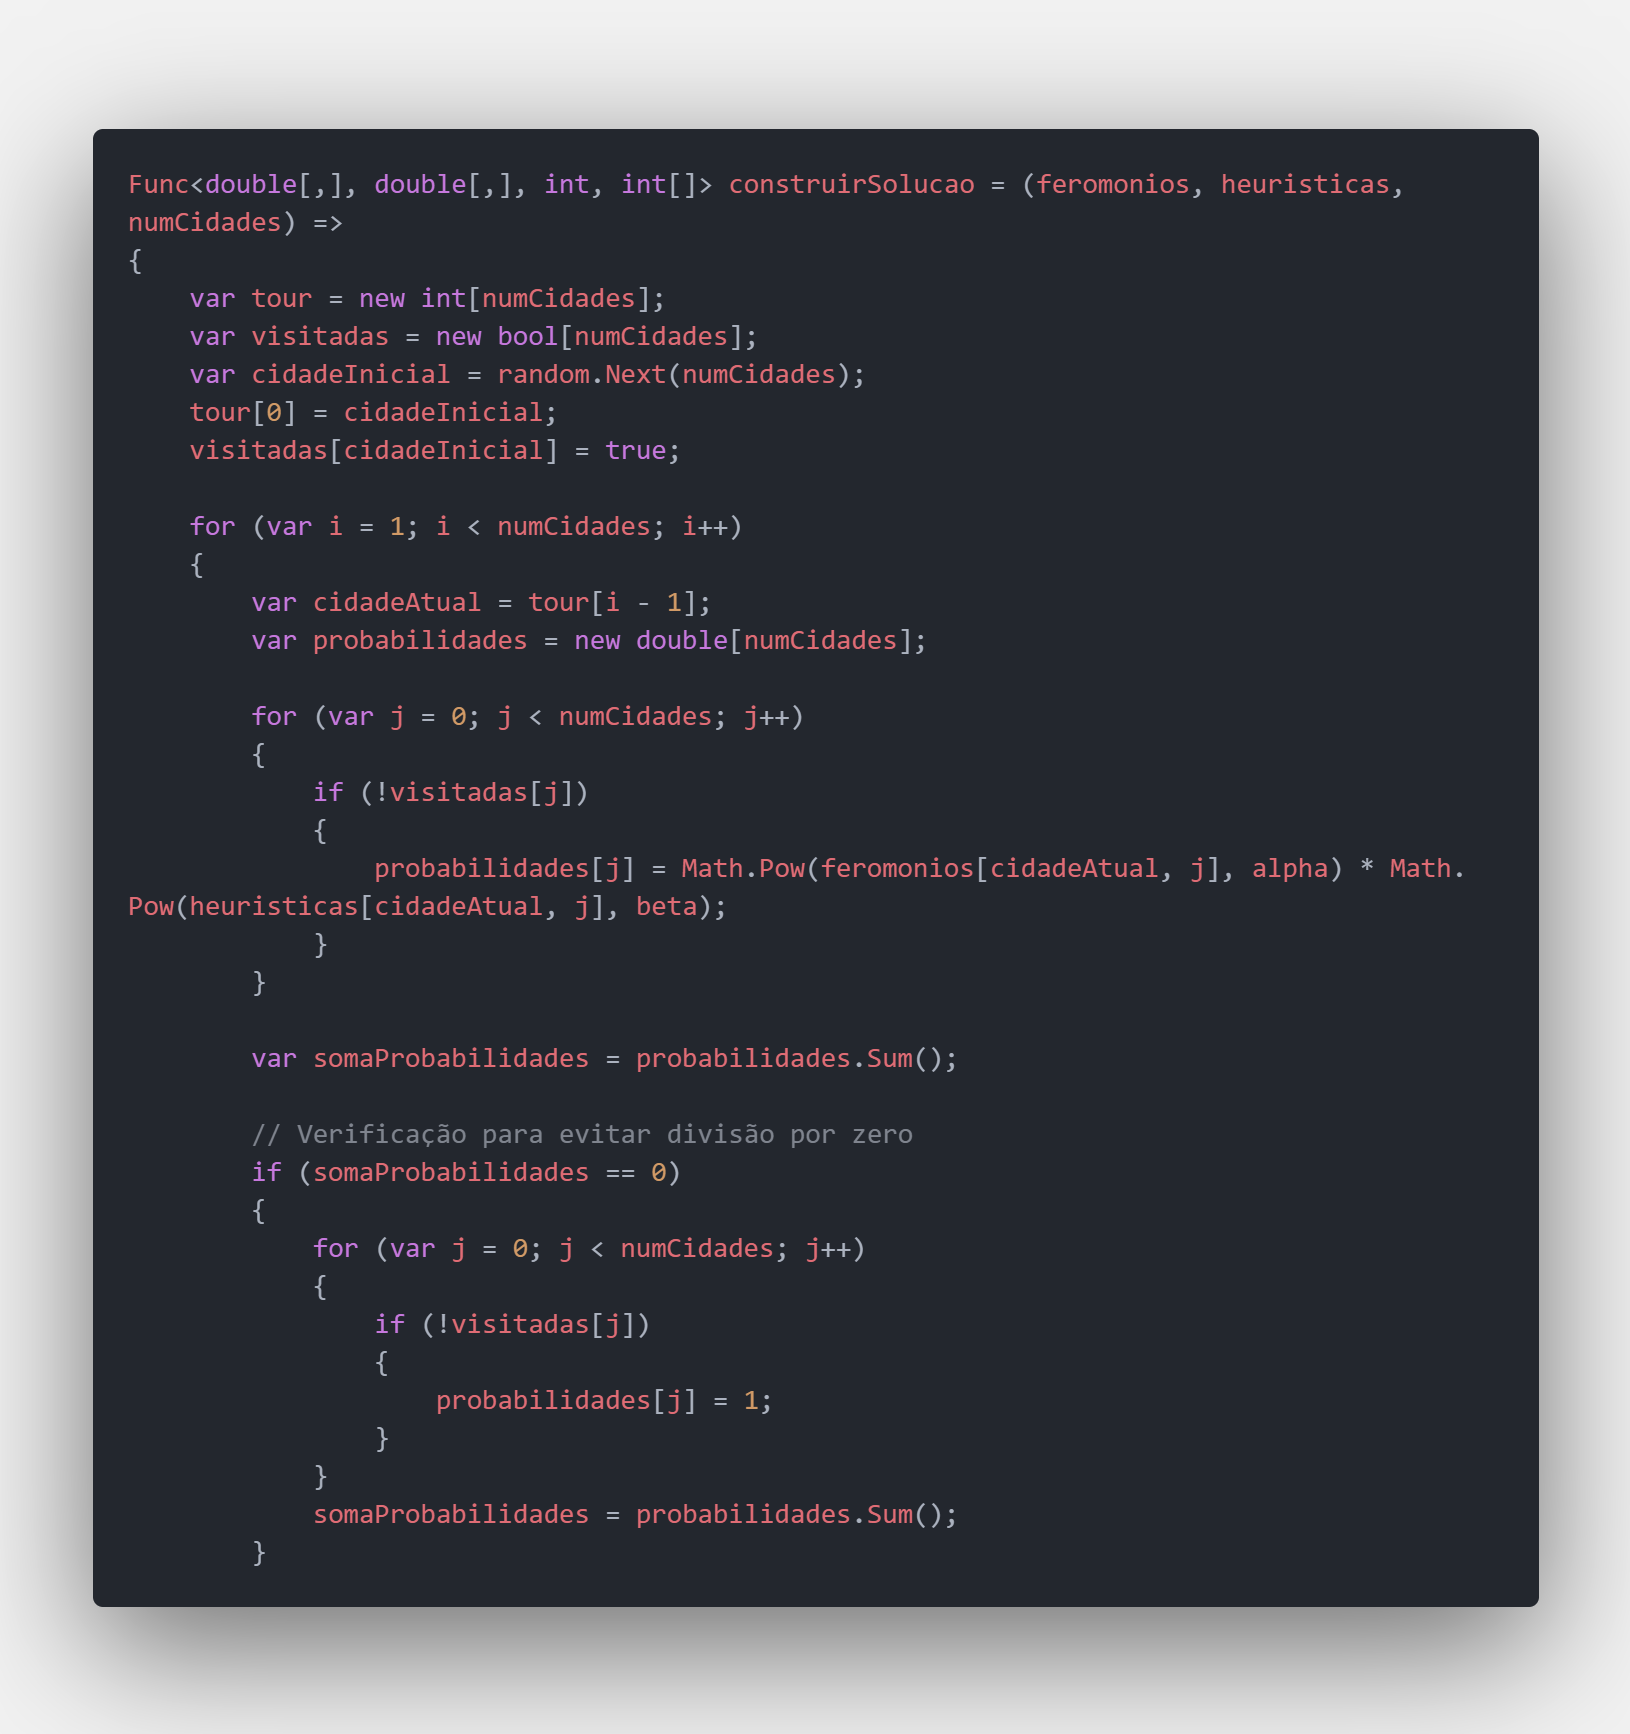
\includegraphics[width=.6\linewidth]{code 1.png} % Substitua "execution_times.png" pelo caminho da sua imagem
			\caption{Construção da solução - primeira parte}
		\end{figure}
	\end{frame}
	
	\begin{frame}
		\frametitle{Solução}
		\begin{figure}
			\centering
			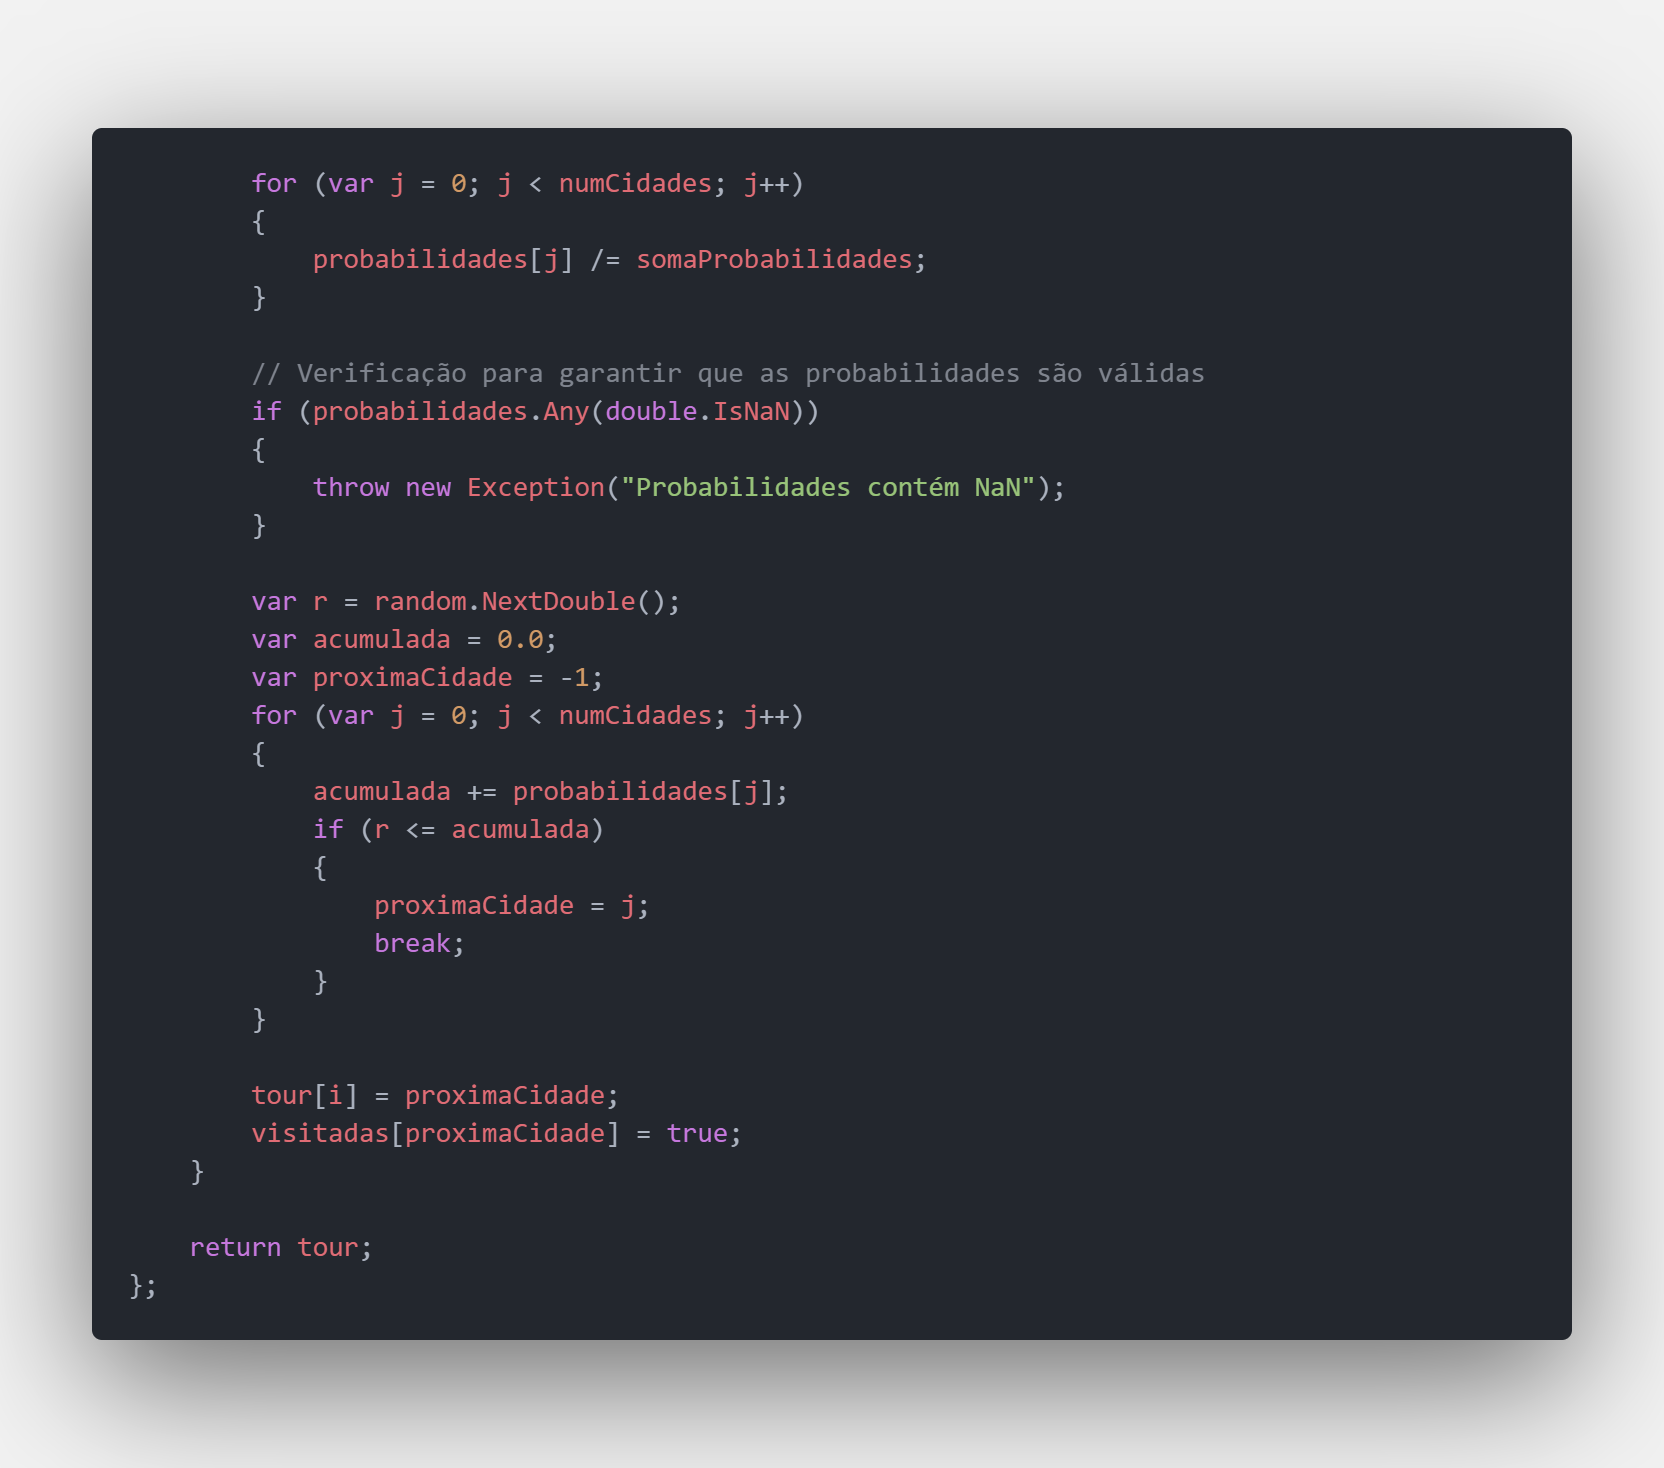
\includegraphics[width=.7\linewidth]{code 2.png} % Substitua "execution_times.png" pelo caminho da sua imagem
			\caption{Construção da solução - segunda parte}
		\end{figure}
	\end{frame}
	
	\begin{frame}
		\frametitle{Solução}
		\begin{figure}
			\centering
			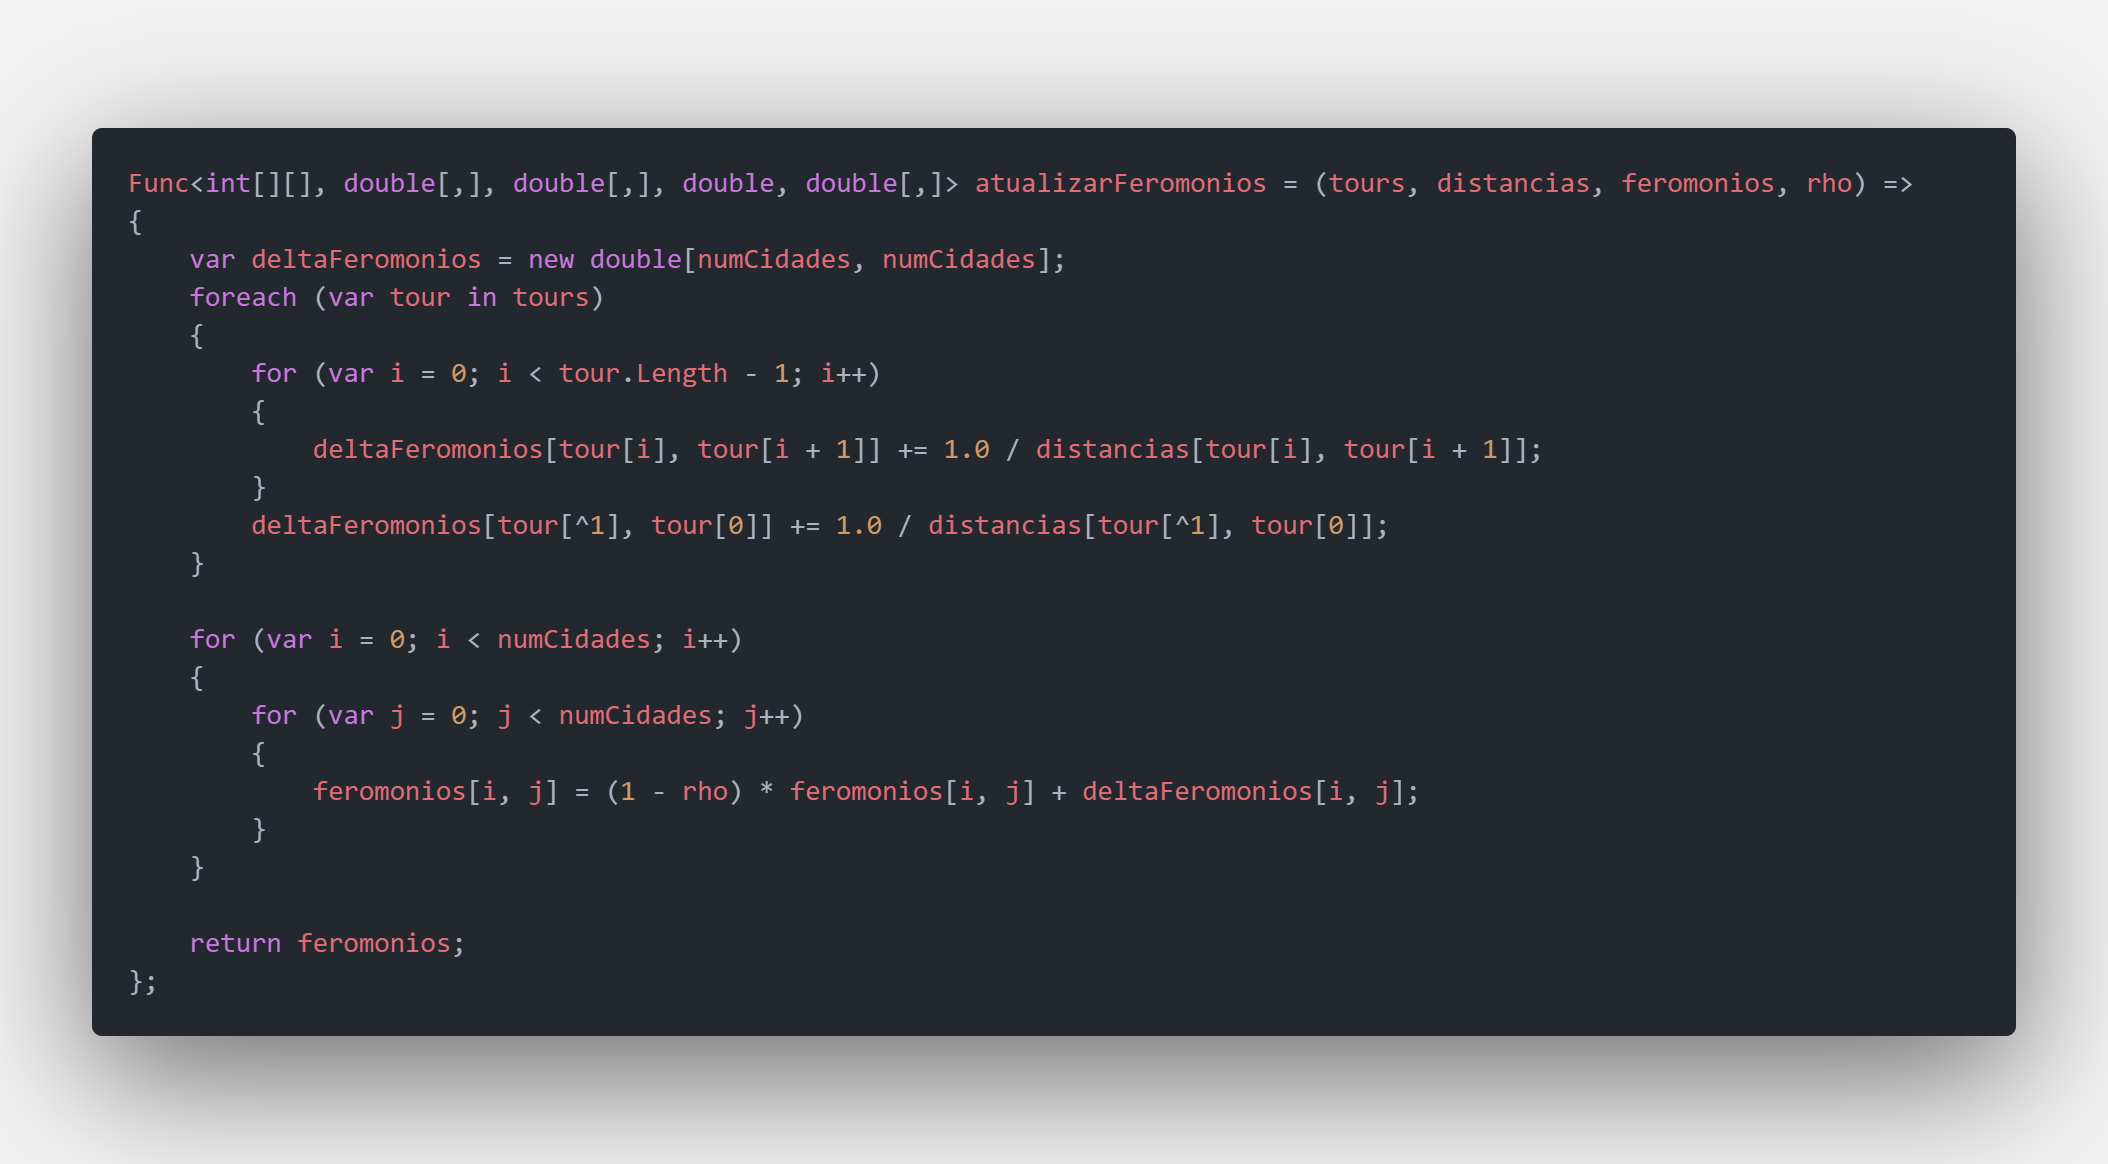
\includegraphics[width=1\linewidth]{code update.png} % Substitua "execution_times.png" pelo caminho da sua imagem
			\caption{Atualização dos feromônios}
		\end{figure}
	\end{frame}
	
	\begin{frame}
		\frametitle{Solução}
		\begin{figure}
			\centering
			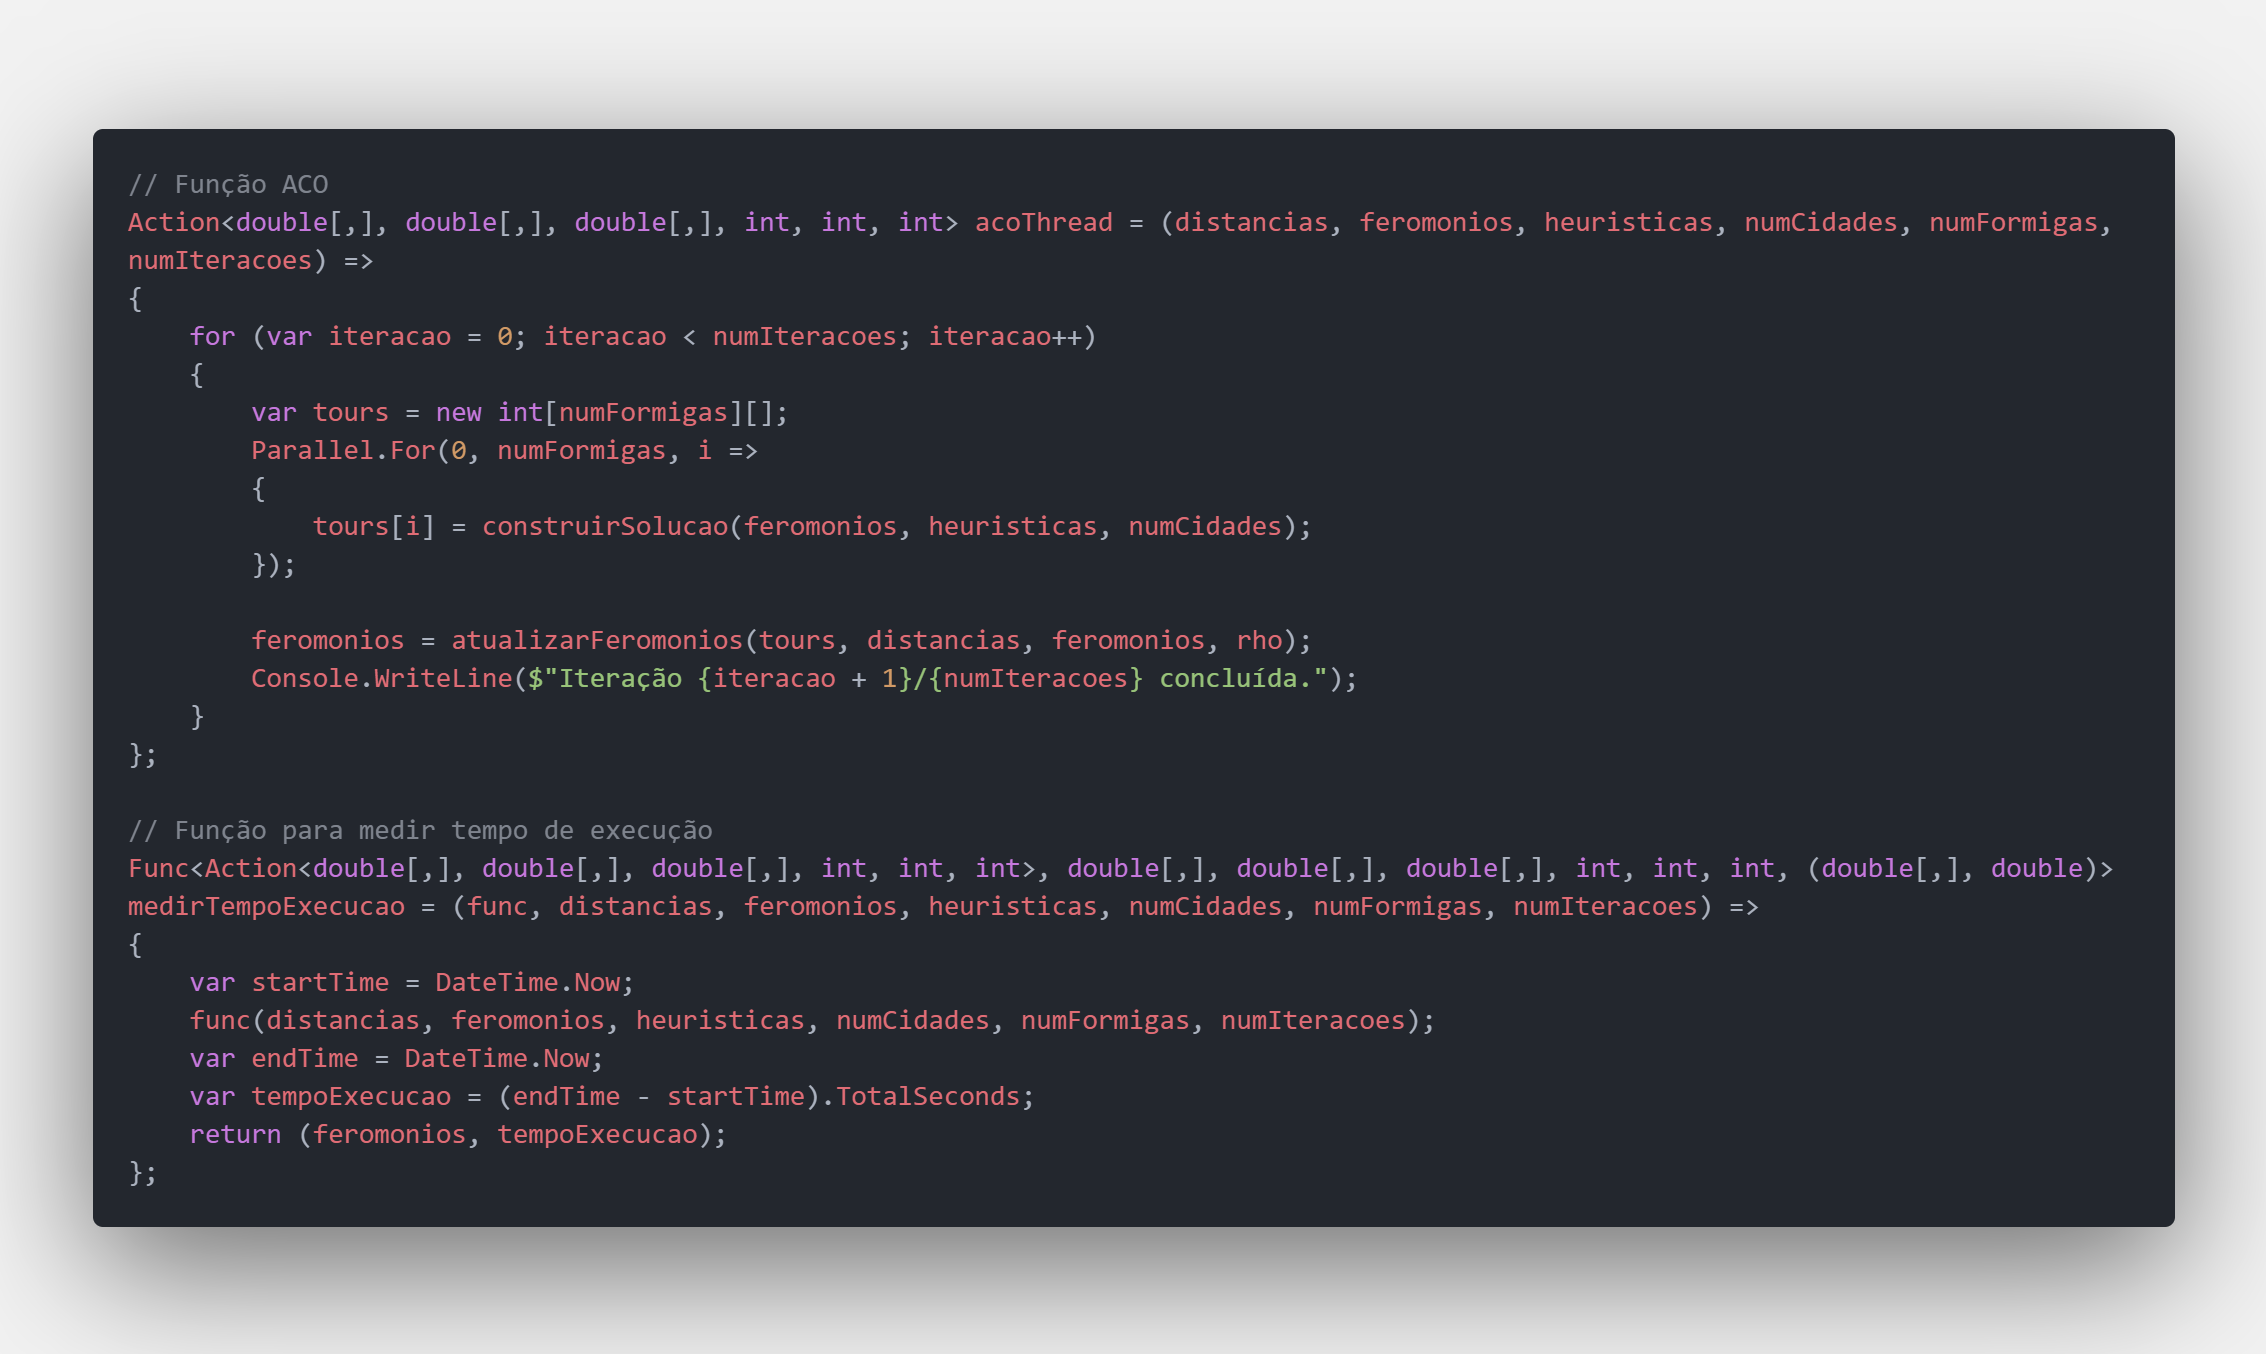
\includegraphics[width=1\linewidth]{code metric.png} % Substitua "execution_times.png" pelo caminho da sua imagem
			\caption{Chamada e medição do tempo de execução}
		\end{figure}
	\end{frame}
	
	\begin{frame}
		\frametitle{Utilização CPU Paralelo}
		\begin{figure}
			\centering
			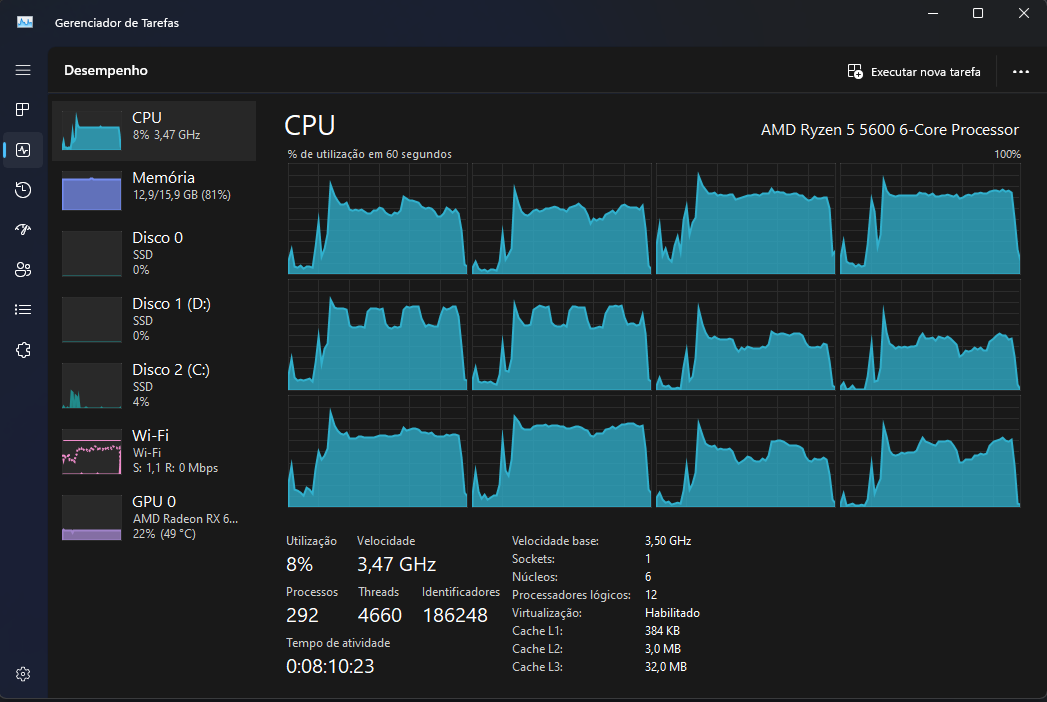
\includegraphics[width=.8\linewidth]{CPU Paralelo.png} % Substitua "execution_times.png" pelo caminho da sua imagem
			\caption{Utilização do CPU Paralelo}
		\end{figure}
	\end{frame}
	
	\begin{frame}
		\frametitle{Resultados}
		\begin{itemize}
			\item Comparação entre o algoritmo sequencial e o paralelo.
			\item Medição de tempos de execução e speedup.
		\end{itemize}
	\end{frame}
	
	\begin{frame}
		\frametitle{Comparação de Speedup}
		\begin{figure}
			\centering
			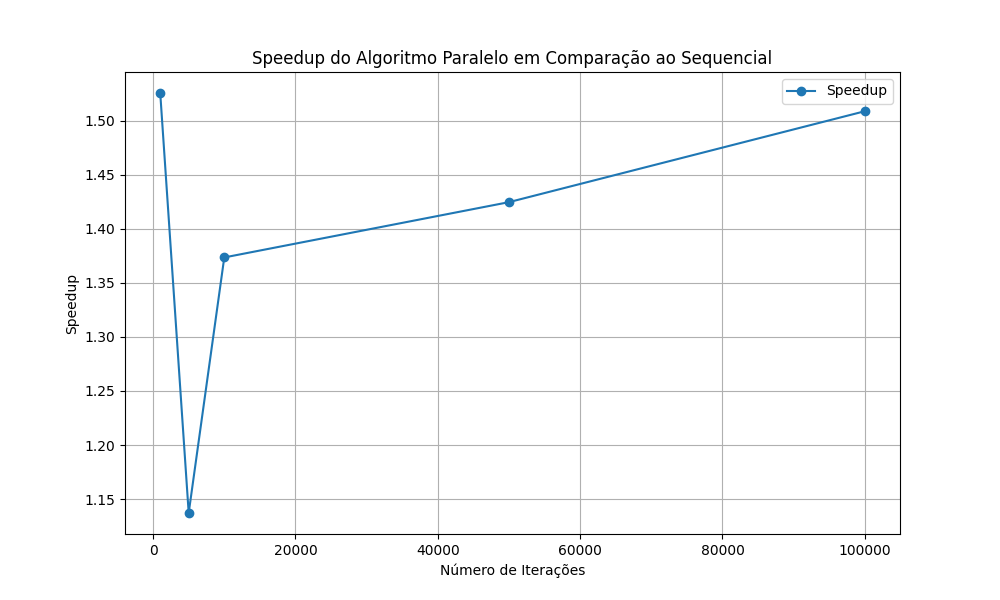
\includegraphics[width=1\linewidth]{speedup.png} % Substitua "speedup.png" pelo caminho da sua imagem
			\caption{Comparação de Speedup}
		\end{figure}
	\end{frame}
	
	\begin{frame}
		\frametitle{Comparação de Tempos de Execução}
		\begin{figure}
			\centering
			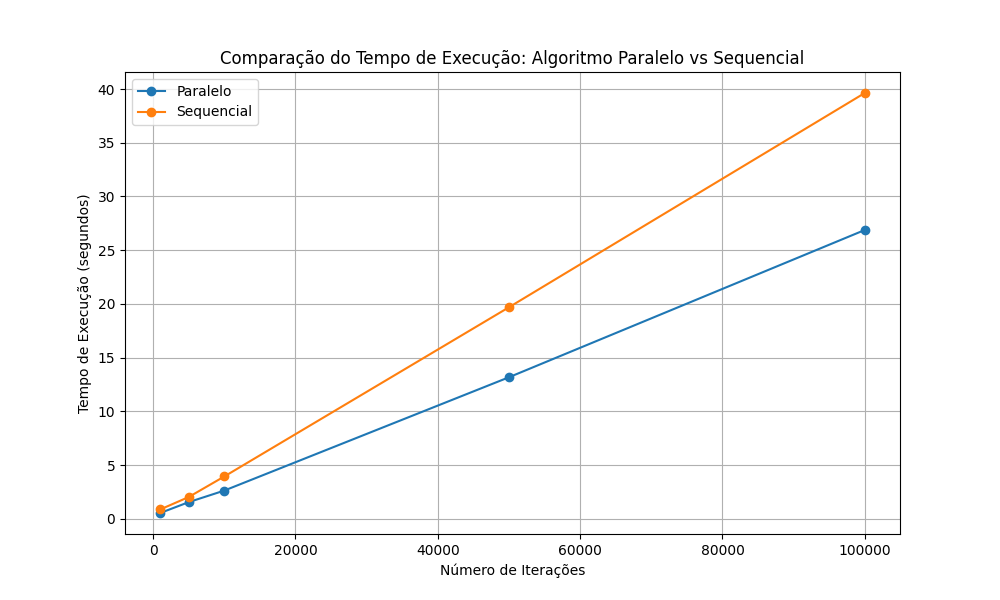
\includegraphics[width=1\linewidth]{comparacao_tempo_execucao.png} % Substitua "execution_times.png" pelo caminho da sua imagem
			\caption{Comparação de Tempos de Execução}
		\end{figure}
	\end{frame}
	
	\begin{frame}
		\frametitle{Conclusão}
		\begin{itemize}
			\item O modelo proposto de ACO paralelo em CPUs multi-core mostrou uma aceleração significativa em comparação com a versão sequencial.
			\item A abordagem VRW e a utilização de instruções vetoriais melhoraram a eficiência da construção do tour.
			\item Resultados indicam o potencial de CPUs multi-core para resolver problemas de grande escala de forma eficiente.
		\end{itemize}
	\end{frame}
	
\end{document}
